\chapter{Configuraciones Realizadas en el Proyecto}
\begin{table}[htb]
\footnotesize
\begin{tabular}{|c|}
\hline
\textbf{Configuraciones Realizadas}\\
\hline
Creaci'on de Organizaciones de Ventas, Canales de Distribuci'on y Sectores\\
\hline
Creaci'on de Oficinas de Ventas y 'Areas de Ventas\\
\hline
 Asignar las Organizaciones de Ventas creadas a la Sociedad\\
\hline
Asignar los Canales de Distribuci'on a las Organizaciones de Ventas\\
\hline
Asignar los Sectores a las Organizaciones de Ventas \\
\hline
Asignar las Oficinas de Ventas a las 'Areas de Ventas\\
\hline
Asignar las Organizaciones de Ventas y Canales de Distribuci'on a los Centros de Distribuci'on\\
\hline
Asignar los Puestos de Expedici'on a los Centros de Distribuci'on\\
\hline
\end{tabular}
\caption{Configuraciones realizadas para establecer la relaci'on entre las distintas unidades componentes de la estructura de SSA Beverage}
\label{tb:asignaciones}
\end{table}
\section{Configuraci'on de la Estructura de SSA Beverage}
	En esta secci'on se presentan las im'agenes de la estructura resultante de la segunda fase del desarrollo del proyecto.
\begin{figure}[H]
\centering
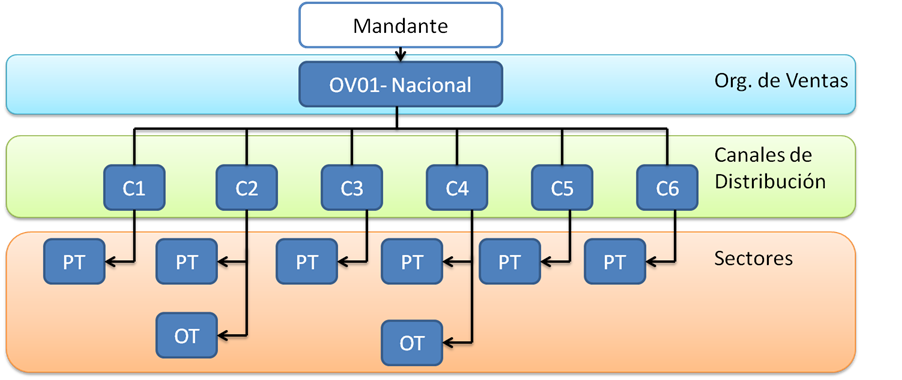
\includegraphics[scale=0.65,type=png,ext=.png,read=.png]{figures/Org1}
\caption{Estructura de SSA Beverage resultante de la Fase del Blueprint}
\label{fig:estructura1}
\end{figure}
\begin{figure}[H]
\centering
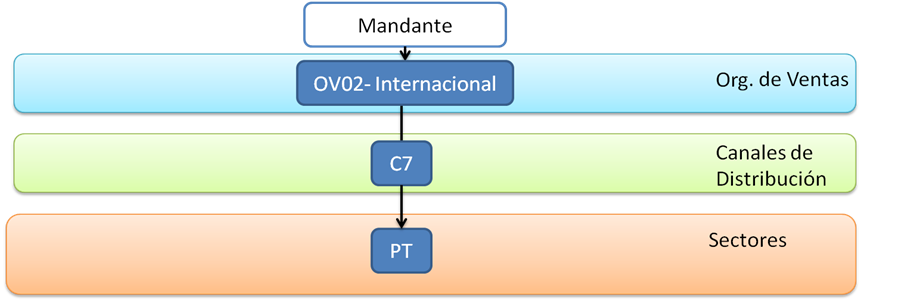
\includegraphics[scale=0.65,type=png,ext=.png,read=.png]{figures/Org2}
\caption{Estructura de SSA Beverage resultante de la Fase del Blueprint - Parte 2}
\label{fig:estructura2}
\end{figure}

	A continuaci'on, se muestra las configuraciones realizadas sobre la estructura de la empresa dentro de SAP SD.
	
	\subsection*{Creaci'on de las Organizaciones de Ventas}
\begin{figure}[H]
\centering
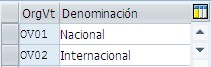
\includegraphics[scale=0.65,type=jpg,ext=.jpg,read=.jpg]{figures/OrgVentas}
\caption{Organizaciones de Ventas}
\label{fig:organizaciones}
\end{figure}

\subsection*{Creaci'on de los Canales de Distribuci'on}
\begin{figure}[H]
\centering
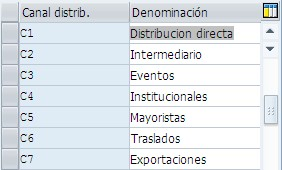
\includegraphics[scale=0.65,type=jpg,ext=.jpg,read=.jpg]{figures/CanalesDistribucion}
\caption{Canales de Distribuci'on}
\label{fig:canales}
\end{figure}

\subsection*{Creaci'on de los Sectores}
\begin{figure}[H]
\centering
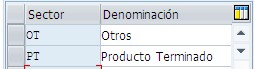
\includegraphics[scale=0.65,type=jpg,ext=.jpg,read=.jpg]{figures/Sectores}
\caption{Sectores}
\label{fig:sectores}
\end{figure}

\subsection*{Creaci'on de las 'Areas de Ventas}
\begin{figure}[H]
\centering
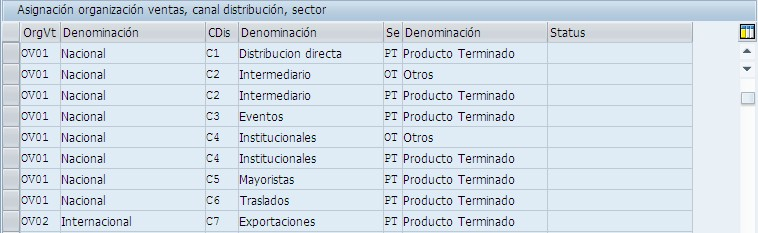
\includegraphics[scale=0.65,type=jpg,ext=.jpg,read=.jpg]{figures/AreaVentas}
\caption{'Areas de Ventas}
\label{fig:areas}
\end{figure}

\subsection*{Creaci'on de las Oficinas de Ventas}
\begin{figure}[H]
\centering
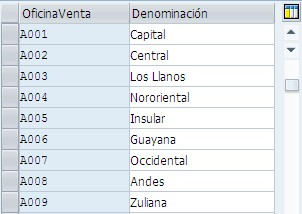
\includegraphics[scale=0.65,type=jpg,ext=.jpg,read=.jpg]{figures/OfVenta}
\caption{Oficinas de Ventas}
\label{fig:oficinas}
\end{figure}

\subsection*{Parte de la creaci'on de los Puestos de Carga}
\begin{figure}[htb]
\centering
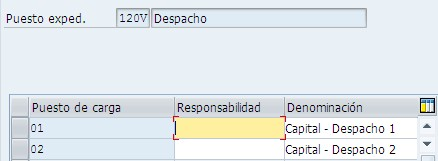
\includegraphics[scale=0.65,type=jpg,ext=.jpg,read=.jpg]{figures/PuestoCarga}
\caption{Parte de los Puestos de Carga definidos para el M'odulo SD}
\label{fig:carga}
\end{figure}

	En las configuraciones sucesivas de esta secci'on, lo que se realiz'o fue el establecimiento de las relaciones entre las distintas componentes de la empresa.

\subsection*{Asignaci'on de las Organizaciones de Venta a los Canales de Distribuci'on}	
\begin{figure}[H]
\centering
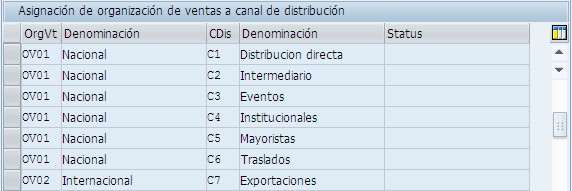
\includegraphics[scale=0.65,type=jpg,ext=.jpg,read=.jpg]{figures/OrgVentasCanales}
\caption{Asignaci'on de las Organizaciones de Ventas a los Canales de Distribuci'on}
\label{fig:asigna2}
\end{figure}

\subsection*{Asignaci'on de las Organizaciones de Ventas a los Sectores creados}
\begin{figure}[H]
\centering
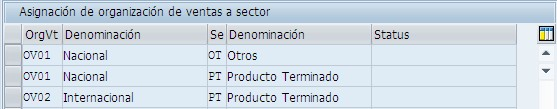
\includegraphics[scale=0.65,type=jpg,ext=.jpg,read=.jpg]{figures/OrgVentasSector}
\caption{Asignaci'on de las Organizaciones de Ventas a los Sectores}
\label{fig:asigna3}
\end{figure}

\subsection*{Asignaci'on de las Oficinas de Ventas a las 'Areas de Ventas}
\begin{figure}[H]
\centering
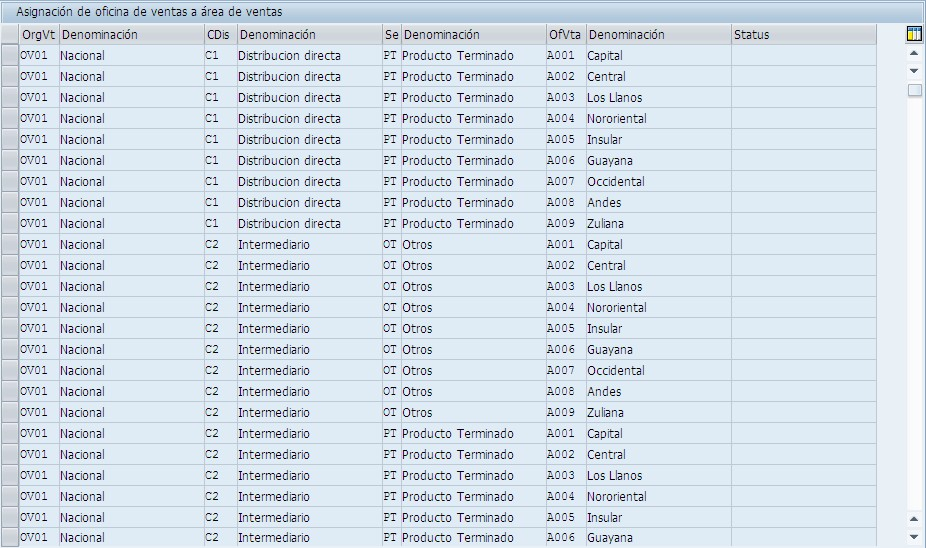
\includegraphics[scale=0.65,type=jpg,ext=.jpg,read=.jpg]{figures/OfVentaAreas}
\caption{Parte de la asignaci'on de las Oficinas de Ventas a las 'Areas de Ventas}
\label{fig:asigna4}
\end{figure}

\subsection*{Asignaci'on de las Organizaciones de Ventas y Canales de Distribuci'on a los Centros de Distribuci'on}
\begin{figure}[H]
\centering
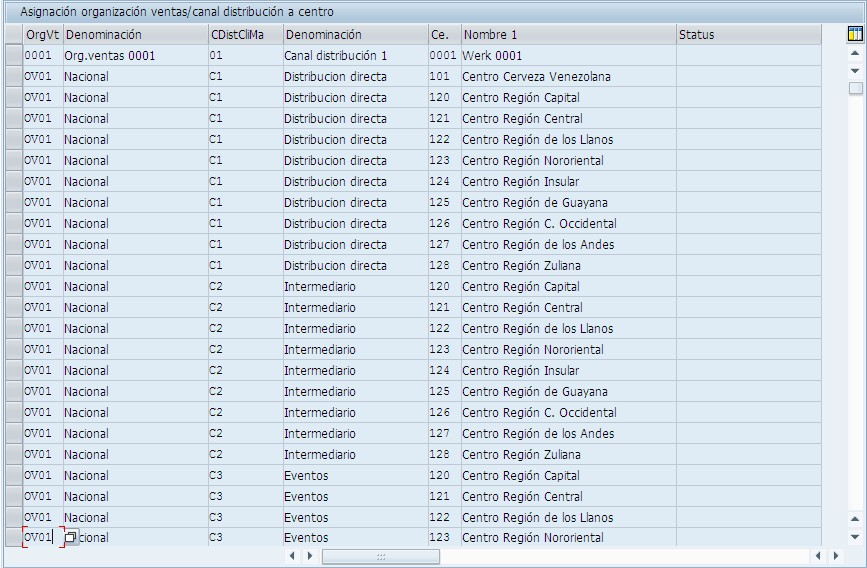
\includegraphics[scale=0.65,type=jpg,ext=.jpg,read=.jpg]{figures/OrgCanalCentro}
\caption{Parte de la asignaci'on de las Orgnanizaciones de Ventas y Canales de Distribuci'on a los Centros de Distribuci'on}
\label{fig:asigna5}
\end{figure}

\subsection*{Parte de la asignaci'on de los Puestos de Expedici'on a los Centros de Distribuci'on}
\begin{figure}[htb]
\centering
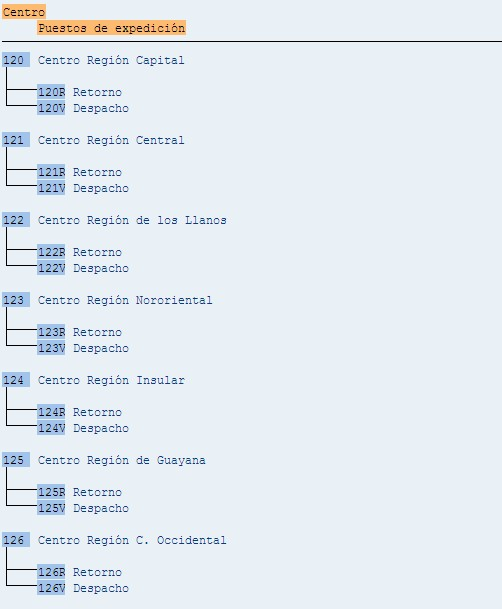
\includegraphics[scale=0.65,type=jpg,ext=.jpg,read=.jpg]{figures/ExpedicionCentro}
\caption{Parte de la asignaci'on de los Puestos de Expedici'on a los Centros de Distribuci'on}
\label{fig:asigna6}
\end{figure}

\section{Ciclo de Ventas presentado en la 'Ultima Fase del Desarrollo}
\begin{table}[h!]
\footnotesize
\scalebox{0.8} {
\begin{tabular}{l l l}
\toprule
\textbf{Nombre de la Transacci'on:} & VA01 &\\
\midrule
                 & \textbf{Clase de Pedido:} & ZSSA (Pedido Est'andar SSA Beverage) \\
                 \cmidrule{2-3}
                 & \textbf{Organizaci'on de Ventas:} & OV01 (Nacional) \\
                 \cmidrule{2-3}
                 & \textbf{Canal de Distribuci'on:} & C1 (Distribuci'on Directa) \\
                 \cmidrule{2-3}
                 & \textbf{Sector:}                   &   PT (Productos Terminados) \\
                 \cmidrule{2-3}
                 & \textbf{Pedido de Venta:}            & 21 \\
                 \cmidrule{2-3}
                 & \textbf{Solicitante:}              & 12 (DYM3000 C.A \\
                \cmidrule{2-3}
  \textbf{Datos de la Transacci'on:}              & \textbf{Dest. Mercanc'ia:}   &   12 (DYM3000 C.A \\
                 \cmidrule{2-3}
                 & \textbf{Nro. Pedido Cliente:} & 58      \\
                 \cmidrule{2-3}
                 & \textbf{Fecha de Pedido:} & 19.09.2013 \\
                 \cmidrule{2-3}
                 & \textbf{Bloqueo de Entrega:}  &      \\
                 \cmidrule{2-3}
                 & \textbf{Material:} & 84000001 (Refresco Lim'on Soda) \\
                 \cmidrule{2-3}
                 & \textbf{Cantidad de pedido} & 1 \\
                 \cmidrule{2-3}
                 & \textbf{Unidad de Pedido} & CAJ (Cajas) \\
                 \midrule
                 & \textbf{Resultado Obtenido:} & Exitoso \\
                 \cmidrule{2-3}
\textbf{Resultados de la Transacci'on:}    & \textbf{N'umero de Pedido arrojado por SAP:} & 00000021 \\
                 \cmidrule{2-3}
                 & \textbf{Observaciones:} &  \\
                 \bottomrule
\end{tabular}}
\caption{Proceso de Pedido de Venta presentado}
\label{tb:pedido}
\end{table}

\begin{table}[h!]
\footnotesize
\scalebox{0.8} {
\begin{tabular}{l l l}
\toprule
\textbf{Nombre de la Transacci'on:} & VL01N &\\
\midrule
                 & \textbf{Pedido:} & 00000021 \\
                 \cmidrule{2-3}
                 & \textbf{Puesto de Expedici'on:} & 120V (Despacho) \\
                 \cmidrule{2-3}
                 & \textbf{Centro de Distribuci'on:} & 120 (Regi'on Capital) \\
                 \cmidrule{2-3}
\textbf{Datos de la Transacci'on:}                  & \textbf{Almac'en:}                   &   PT01 \\
                 \cmidrule{2-3}
                 & \textbf{Cantidad Picking:}            & 1 \\
                 \cmidrule{2-3}
                 & \textbf{Unidad Picking:}              & CAJ (Cajas) \\
                 \midrule
                 & \textbf{Resultado Obtenido:} & Exitoso \\
                 \cmidrule{2-3}
\textbf{Resultados de la Transacci'on:}    & \textbf{N'umero de Entrega arrojado por SAP:} & 80000008 \\
                 \cmidrule{2-3}
                 & \textbf{Observaciones:} &  Para concluir la Entrega se procedi'o a Contabilizar \\
                 &                                      & el Material (Contabilizar SM) y fue exitoso\\
                 \bottomrule
\end{tabular}}
\caption{Proceso de Entrega presentado}
\label{tb:entrega}
\end{table}

\begin{table}[h!]
\footnotesize
\scalebox{0.8} {
\begin{tabular}{l l l}
\toprule
\textbf{Nombre de la Transacci'on:} & VF01 &\\
\midrule
                 & \textbf{N'umero de Documento:} &  80000008 \\
                 \cmidrule{2-3}
  \textbf{Datos de la Transacci'on:}                  & \textbf{Clase de Factura:} & Factura SSA Beverage \\
                 \midrule
                 & \textbf{Resultado Obtenido:} & Exitoso \\
                 \cmidrule{2-3}
\textbf{Resultados de la Transacci'on:}    & \textbf{N'umero de Factura arrojado por SAP:} & 90000007 \\
                 \cmidrule{2-3}
                 & \textbf{Observaciones:} &  Para concluir la Factura se procedi'o a Autorizar \\
                 &                                      & Contabilizaci'on (Esto es para crear Documento \\
                 &                                      & Contable) y fue exitoso\\
                 \bottomrule
\end{tabular}}
\caption{Proceso de Facturaci'on presentado}
\label{tb:facturacion}
\end{table}